\documentclass{article}
\usepackage[left=2cm, right=2cm, top=2cm]{geometry}
%%%%%%%%%%%%%%%%%%%%%%%%%%%%%%%%%% PACKAGES %%%%%%%%%%%%%%%%%%%%%%%%%%%%%%%%%%
\usepackage{minted}                     % Code
\usepackage{graphicx}                   % PNGs
\usepackage{hyperref}                   % Hyperlinks
\hypersetup{
    colorlinks,
    linkcolor=black
}

%%%%%%%%%%%%%%%%%%%%%%%%%%%%%%%%%%%%%%%%%%%%%%%%%%%%%%%%%%%%%%%%%%%%%%%%%%%%%%%

\pagenumbering{gobble}

\title{\textbf{Homework #1}}
\author{MacMillan, Kyle}
\date{September 28, 2018}


\begin{document}

\maketitle
\addcontentsline{toc}{section}{Title}

\newpage
\pagenumbering{roman}   % Set TOC page numbering to lowercase roman numerals
\tableofcontents
\addcontentsline{toc}{section}{Table of Contents}


\newpage
\listoffigures
\addcontentsline{toc}{section}{\listfigurename}


\newpage
\pagenumbering{arabic}  % Set content page numbering to arabic numerals
% Setup Hyperlinks for the rest of the document
\hypersetup{
    colorlinks,
    citecolor=blue,
    filecolor=black,
    linkcolor=blue,
    urlcolor=blue
}

\section{Problem 1}}
\setcounter{page}{1} % Set the page counter to 3
\textit{What are the identity values for the operators}: $\&\&,\ ||,\ |,\ ^\wedge $?

\begin{itemize}
    \begin{tabular}{@{}ll}
    \item $\&\&$ &: 1\\
    \item $||$ &: 0\\
    \item $|$ &: 0\\
    \item $^\wedge$ &: 0\\
    \end{tabular}
\end{itemize}



\section{Problem 2}
\textit{Suppose OpenMP did not have the reduction clause. Show how to implement an efficient parallel reduction by adding a private variable and using the critical pragma.}
\inputminted{c++}{problem2.cpp}

\begin{figure}[h]
    \centering
    \begin{minipage}{0.7\textwidth}
        \centering
        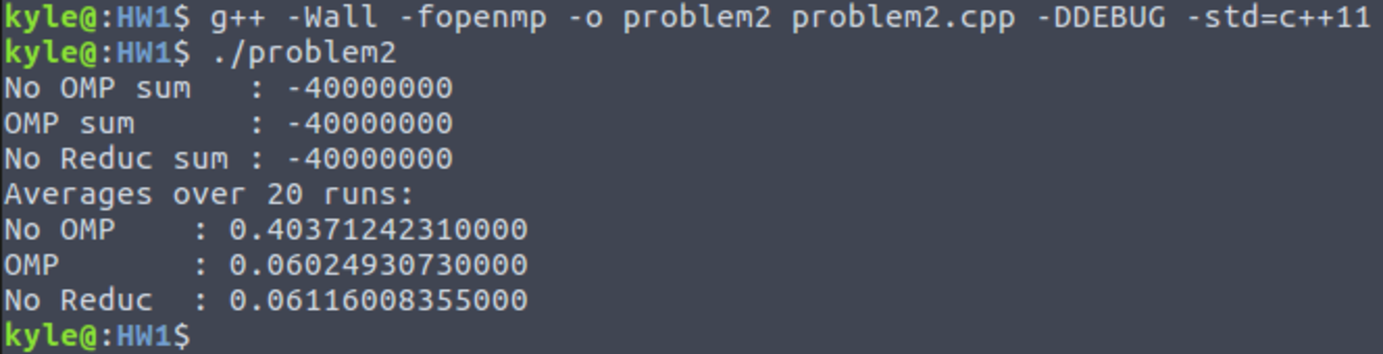
\includegraphics[width=0.95\textwidth]{Problem2debug}
        \caption{Example debug output.}
        \label{fig:p2debug}
    \end{minipage}\hfill
    \begin{minipage}{0.3\textwidth}
        \centering
        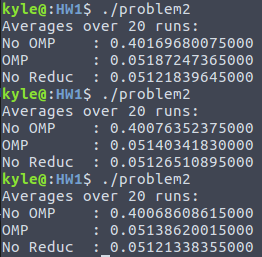
\includegraphics[width=0.95\textwidth]{Problem2_60}
        \caption{Better performance without reduction.}
        \label{fig:p2}
    \end{minipage}
\end{figure}

As can be seen in the figures the sums are performing as expected. An interesting, and expected outcome is that in Figure~\ref{fig:p2debug} it takes 0.06 seconds to run $OMP$ and $No\ Reduc$ but in Figure~\ref{fig:p2} it takes 0.05 seconds. The $No\ OMP$ takes 0.40 seconds regardless. The reason for this behavior is that $OMP$ uses the cores you give it and at the time of recording the first figure the browser was open and running a video. When I recorded the second Figure I had closed my browser to maximize performance for multi-core processing. The $No\ OMP$ section of code was only running on one core, so it did not care that I had a video playing.


\section{Problem 3}
\subsection{Problem 3a}
% \inputminted[linestart=136,lineend=141]{c++}{problem3.cpp}
% TODO: Insert code from 3a

\subsection{Problem 3b}
This code section is not suitable for OpenMP because of the \&\& operator in comparison.
Per the \hyperlink{https://www.openmp.org/wp-content/uploads/openmp-4.5.pdf}{OpenMP documentation} \S2.6, p53:\\\\
\begin{tabular}{@{}ll}
$test$-$expr$ & One of the following:\\
& $var\ relational$-$op\ b$\\
& $b\ relational$-$op\ var$\\\\

$relational$-$op$ & One of the following:\\
& $<$  \\
& $<=$ \\
& $>$  \\
& $>=$ \\
\end{tabular}

\subsection{Problem 3c}
This code can be ran with OMP but it is dependent on whether or not $foo()$ is threadsafe.

\subsection{Problem 3d}
asdf

\subsection{Problem 3e}
asdf

\subsection{Problem 3f}
asdf

\subsection{Problem 3g}
asdf

\subsection{Problem 3h}
asdf



\section{Problem 4}
asdf


\section{Problem 5}
\textit{If the address of the nodes in a hypercube has n bits. How many nodes can it be at the most and how many edges does each node have? 
Give an algorithm that routes a message from node u to node v in this k-node hypercube in no more than log(k) steps.}


\section{Graduate Assignment}
asdf


\end{document}
